\documentclass[12pt,a4paper,onecolumn]{article}
\usepackage[utf8]{inputenc}
\usepackage[T1]{fontenc}
\usepackage[french]{babel}

% ------------------------- Color table ----------------------------------------
\usepackage{multirow}
\usepackage[table]{xcolor}
\definecolor{maroon}{cmyk}{0,0.87,0.68,0.32}
% ------------------------------------------------------------------------------

\usepackage{amscd}
\usepackage{amsthm}
\usepackage{physics}
\usepackage[left=2.2cm,right=2.2cm,top=2cm,bottom=2cm]{geometry}
\usepackage{textcomp,gensymb} %pour le °C, et textcomp pour éviter les warning
\usepackage{graphicx} %pour les images
\usepackage{caption}
\usepackage{subcaption}
\usepackage[colorlinks=true,
	breaklinks=true,
	citecolor=blue,
	linkcolor=blue,
	urlcolor=blue]{hyperref} % pour insérer des liens
\usepackage{epstopdf} %converting to PDF
\usepackage[export]{adjustbox} %for large figures

\usepackage{array}
\usepackage{dsfont}% indicatrice : \mathds{1}


% -------------------------- Mathematics ---------------------------------------
\graphicspath{{images/}} % For the images path
% ------------------------------------------------------------------------------

% -------------------------- Mathematics ---------------------------------------
\usepackage{mathrsfs, amsmath, amsfonts, amssymb}
\usepackage{bm}
\usepackage[Symbol]{upgreek} % For pi \uppi different from /pi
\newcommand{\R}{\mathbb{R}} % For Real space
% ------------------------------------------------------------------------------


% -------------------------- Code format ---------------------------------------
\usepackage[numbered,framed]{matlab-prettifier}
\lstset{
	style              = Matlab-editor,
	basicstyle         = \mlttfamily,
	escapechar         = '',
	mlshowsectionrules = true,
}
% ------------------------------------------------------------------------------

% ------------------------- Blbiographie --------------------------------------
% \usepackage[backend=biber, style=science]{biblatex}
% \addbibresource{biblio.bib}
% ------------------------------------------------------------------------------


\setcounter{tocdepth}{4} %Count paragraph
\setcounter{secnumdepth}{4} %Count paragraph
\usepackage{float}

\usepackage{graphicx} % for graphicspath
% \graphicspath{{../images/}}

\usepackage{array,tabularx}
\newcolumntype{L}[1]{>{\raggedright\let\newline\\\arraybackslash\hspace{0pt}}m{#1}}
\newcolumntype{C}[1]{>{\centering\let\newline\\\arraybackslash\hspace{0pt}}m{#1}}
\newcolumntype{R}[1]{>{\raggedleft\let\newline\\\arraybackslash\hspace{0pt}}m{#1}}


% ------------------------------ TITLE -----------------------------------------
\title{Math M2 Probabilistic graphical models 2017/2018}
\author{Vincent Matthys}
% ------------------------------------------------------------------------------

% ------------------------------ NUMEROTATION ----------------------------------
% \renewcommand{\thesubsection}{\alph{subsection}}
% ------------------------------------------------------------------------------


\begin{document}
\begin{tabularx}{0.8\textwidth}{@{} l X r @{} }
	{\textsc{Master MVA}}                   &  & \textsc{Homework 1} \\
	\textsc{Probabilistic graphical models} &  & {Vincent Matthys}   \\
\end{tabularx}
\vspace{1.5cm}
\begin{center}
	\rule[11pt]{5cm}{0.5pt}

	\textbf{\LARGE \textsc{Compte-rendu du devoir 1}}
	\vspace{0.5cm}\\
	Vincent Matthys\\
	\rule{5cm}{0.5pt}
	\vspace{1.5cm}
\end{center}

\section{Leaning in discrete graphical models}

Etant donné que \(z\) et \(x\) sont des variables à valeurs discrètes prenant respectivement \(M\) et \(K\) valeurs, on peut procéder au \textit{one hot encoding}, notant respectivement \(\bm{Z}\) et \(\bm{X}\) leur encodage sur, respectivement \(\R^M\) et \(\R^K\). Ainsi, on peut écrire :

\[
	p(z = m) = P(Z_m = 1) = \pi_m
\]
\[
	p(x = k | z = m) = p(X_k = 1 | Z_m = 1) = \theta_{mk}
\]
En supposant que l'on ait un échantillon de \(n\) observations de \((x, z)\), on peut exprimer la probabilité jointe d'une obersvation \(i\) :

\begin{equation}
	\begin{split}
		p(x^{(i)}, z^{(i)} ; \bm{\pi}, \bm{\theta}) & = p(z^{(i)} ; \bm{\pi}) p(x^{(i)} | z^{(i)} ; \bm{\theta})                                          \\
		p(x^{(i)}, z^{(i)} ; \bm{\pi}, \bm{\theta}) & = \prod_{m=1}^M \prod_{k=1}^K \theta_{mk}^{X_k^{(i)} Z_m^{(i)}} \prod_{l = 1}^M\pi_l^{Z_l^{(i)}}
	\end{split}
	\label{1_joint}
\end{equation}

On peut alors écrire la log-vraisemblance de l'échantillon dans le modèle \(( \bm{\pi}, \bm{\theta})\), composé d'observations i.i.d., en utilisant~\eqref{1_joint}:

\begin{equation}
	\begin{split}
		\ell( \bm{\pi}, \bm{\theta}) & = \sum_{i = 1}^n \ln(p(x^{(i)}, z^{(i)} ; \bm{\pi}, \bm{\theta}))                                                                        \\
		& = \sum_{i = 1}^n\left(\ln\left(\prod_{m=1}^M \prod_{k=1}^K \theta_{mk}^{X_k^{(i)} Z_m^{(i)}} \prod_{l = 1}^M\pi_l^{Z_l^{(i)}}\right)\right)                   \\
		& = \sum_{i = 1}^n\left(\sum_{m=1}^M \sum_{k=1}^K \ln(\theta_{mk}^{X_k^{(i)} Z_m^{(i)}}) + \sum_{l = 1}^M\ln(\pi_l^{Z_l^{(i)}})\right)                          \\
		& = \sum_{i = 1}^n\left(\sum_{m=1}^M \sum_{k=1}^K X_k^{(i)} Z_m^{(i)}\ln(\theta_{mk}) + \sum_{l = 1}^M {Z_l^{(i)}}\ln(\pi_l)\right)                             \\
		& = \sum_{m=1}^M \sum_{k=1}^K \left(\sum_{i = 1}^n X_k^{(i)} Z_m^{(i)}\right)\ln(\theta_{mk}) + \sum_{l = 1}^M\left(\sum_{i = 1}^n {Z_l^{(i)}}\right)\ln(\pi_l) \\
		& = \sum_{m=1}^M \sum_{k=1}^K \alpha_{mk}\ln(\theta_{mk}) + \sum_{l = 1}^M \beta_l\ln(\pi_l)
	\end{split}
	\label{1_logl}
\end{equation}

avec
\begin{align*}
	\alpha_{mk} & = \sum_{i = 1}^n X_k^{(i)} Z_m^{(i)} \\
	\beta_l     & = \sum_{i = 1}^n {Z_l^{(i)}}
\end{align*}

D'après~\eqref{1_logl}, la log-vraisemblance est donc strictement concave en chaque composantes de \(\bm{\pi}\) et \(\bm{\theta}\), par combinaison linéaire de logarithmes. D'autre part, on a les contraintes linéaires suivantes :
\begin{equation}
	\begin{split}
		\sum_{m = 1}^M \pi_m - 1 &= 0\\
		\sum_{k = 1}^K \theta_{mk} - 1 &= 0 \,,  \forall m : 1..M
	\end{split}
\end{equation}

On peut donc écrire le Lagrangien, en utilisant les multiplicateurs de Lagrange correspondants, associé au problème de maximisation de la log-vraisemblance~\eqref{1_logl} :

\begin{equation}
	\mathcal{L}(\bm{\pi}, \bm{\theta}, \lambda, \bm{\gamma}) = \sum_{m=1}^M \sum_{k=1}^K \alpha_{mk}\ln(\theta_{mk}) + \sum_{l = 1}^M \beta_l\ln(\pi_l) - \lambda\left(\sum_{m = 1}^K \pi_m - 1\right) - \bm{\gamma}^\intercal \begin{pmatrix}
		\vdots                         \\
		\sum_{k = 1}^K \theta_{mk} - 1 \\
		\vdots
	\end{pmatrix}
	\label{1_lagrang}
\end{equation}

Le problème admet une solution unique, notée \( (\bm{\widehat{\pi_{MLE}}}, \bm{\widehat{\theta_{MLE}}}) \) que l'on trouve par dérivation de~\eqref{1_lagrang}, puisque cette expression est différentiable.

\subsection{Par rapport à \protect\(\pi_m\)}

\[
	\frac{\partial \mathcal{L}(\bm{\pi}, \bm{\theta}, \lambda, \bm{\gamma})}{\partial \pi_m} = \frac{\beta_m}{\pi_m} - \lambda = 0
	\implies \pi_m \propto \beta_m
	\implies \pi_m = \frac{\beta_m}{\sum_{m=1}^M \beta_m}= \frac{\sum_{i = 1}^n {Z_m^{(i)}}}{\sum_{m=1}^M \sum_{i = 1}^n {Z_m^{(i)}}}
\]
D'où finalement :
\begin{equation}
	\left(\widehat{\pi_{MLE}}\right)_m = \frac{1}{n} \sum_{i = 1}^n {Z_m^{(i)}}
	\label{1_pi}
\end{equation}

\subsection{Par rapport à \protect\(\theta_{mk}\)}

\[
	\frac{\partial \mathcal{L}(\bm{\pi}, \bm{\theta}, \lambda, \bm{\gamma})}{\partial \theta_{mk}} = \frac{\alpha_{mk}}{\theta_{mk}} - \gamma_m = 0 \implies \theta_{mk} \propto \alpha_{mk}
	\implies \theta_{mk} = \frac{\alpha_{mk}}{\sum_{k = 1}^K \alpha_{mk}} = \frac{\sum_{i = 1}^n X_k^{(i)} Z_m^{(i)}}{\sum_{i = 1}^n \left(\sum_{k=1}^K X_k^{(i)}\right) Z_m^{(i)}}
\]

D'où finalement :

\begin{equation}
	\left( \widehat{{\theta_{MLE}}} \right)_{mk} = \frac{\sum_{i = 1}^n X_k^{(i)} Z_m^{(i)}}{\sum_{i = 1}^n Z_m^{(i)}}
\end{equation}

On remarque que si \( \sum_{i = 1}^n Z_m^{(i)} \) est nulle, alors \( \left(\widehat{{\theta_{MLE}}}\right)_{mk} \) n'est pas défini, et ce pour tout \( k\). Mais, dans de telles conditions, cela signifie que la \( m \)\up{ième} valeur de \( z \) n'a pas été observée, et donc que l'on peut réduire \( \bm{\theta} \) d'une ligne entière, puisqu'alors la probabilité d'observer une quelconque valeur de \( x\) sachant que \( z\) prend la valeur \( m\) est nulle.

En définitif, on peut s'affranchir de l'hypothèse implicite qu'aucune composante de \(\bm{\pi}\) ni de \(\bm{\theta}\) n'est nulle. En effet, si tel est le cas, alors la probabilité d'observer une telle observation est nulle.

\subsection{Conclusion}
On remarque donc que l'estimateur de \(\bm{\pi}\) n'est rien d'autre que la moyenne empirique des observations de \( z\), et que l'estimateur de \(\bm{\theta}\) est également la moyenne des observations de \( x\) pour une valeur de \( z \) donnée.

\section{Linear classification}

\subsection{Generative model : Linear Discriminant Analysis}

Supposons un échantillon de \( N \) observations de \( x, y \), notées, \( (x_n, y_n) \), pour \( n \) variant de \( 1 \) à \( N \), où \(y_n \in \{0,1\} \). Etant donné le modèle suivant :
\begin{equation*}
	\begin{split}
		y &\sim Bernoulli(\uppi) \\
		p(x | y = i) &= \frac{1}{2\pi\sqrt{\det\Sigma}}\exp\left(-\frac{1}{2}(x - \mu_i)^\intercal\Sigma^{-1}(x - \mu_i)\right)
	\end{split}
\end{equation*}
paramétré par :
\[
	\Theta = (\mu_0, \mu_1, \Sigma, \uppi)
\]
on peut réecrire la probabilité d'observer \( (x_n, y_n )\) sous la forme comprenant déjà la contrainte sur \( \pi \):
\begin{equation}
	p(x_n, y_n) = \left(\uppi p(x_n | y_n = 1)\right)^{y_n} \left((1 - \uppi) p(x_n | y_n = 0)\right)^{1 - y_n}
	\label{2_1_joint}
\end{equation}
ce qui permet de déterminer la log-vraisemblance de l'échantillon composé de \( N \) observations i.i.d dans le modèle \( \Theta \) en utilisant~\eqref{2_1_joint} :
\begin{equation}
	\begin{split}
		\ell(\Theta) & =  \sum_{n = 1}^N \ln(p(x_n, y_n ; \Theta)) \\
		\ell(\Theta) & =  \sum_{n = 1}^N \ln\left(\left(\uppi p(x_n | y_n = 1)\right)^{y_n} \left((1 - \uppi) p(x_n | y_n = 0)\right)^{1 - y_n}\right) \\
		\ell(\Theta) & =  \sum_{n = 1}^N
		\left(y_n \left(\ln
			\left(\frac{\uppi}{2\pi\sqrt{\det\Sigma}}\right) -\frac{1}{2}(x_n - \mu_1)^\intercal\Sigma^{-1}(x_n - \mu_1) \right)\right)\\
		&+ 	\sum_{n = 1}^N\left((1 - y_n)
		\left(\ln
		\left(\frac{1 - \uppi}{2\pi\sqrt{\det\Sigma}}\right) -\frac{1}{2}(x_n - \mu_0)^\intercal\Sigma^{-1}(x_n - \mu_0) \right)\right) \\
		\ell(\Theta) & =  \sum_{n = 1}^N
		\left(y_n \left(\ln
			\uppi - \ln(2\pi) -\frac{1}{2}\ln\det\Sigma -\frac{1}{2}(x_n - \mu_1)^\intercal\Sigma^{-1}(x_n - \mu_1) \right)\right)\\
		&+ 	\sum_{n = 1}^N\left((1 - y_n)
		\left(\ln(1 - \uppi) - \ln(2\pi) -\frac{1}{2}\ln\det\Sigma -\frac{1}{2}(x_n - \mu_0)^\intercal\Sigma^{-1}(x_n - \mu_0) \right)\right)\\
	\end{split}
	\label{2_1_logl}
\end{equation}

\( \ell(\Theta) \) est donc une fonction stricement concave en \( \uppi\) par stricte concavité du logarithme, en \( \mu_0 \) et \( \mu_1 \) par stricte concavité de l'opposé d'une forme quadratique (avec les valeurs propres de  \( \Sigma \) strictement positives), et en \( \Sigma \) par convextié du logdet.
De plus, \( \ell(\Theta) \) est différentiable. Le problème de maximisation \( \ell(\Theta) \) admet une solution unique, notée \( (\widehat{\mu_{0, MLE}}, \widehat{\mu_{1, MLE}}, \widehat{\Sigma_{MLE}}, \widehat{\uppi_{MLE}}) \) que l'on trouve par dérivation de~\eqref{2_1_logl}.

\subsubsection{Calcul du MLE}
\paragraph*{Par rapport à \protect \(\uppi \)}

\[
	\frac{\partial \ell(\mu_0, \mu_1, \Sigma, \uppi)}{\partial \uppi} = 	\sum_{n = 1}^N\left( \frac{y_n}{\uppi} - \frac{1 - y_n}{1 - \uppi} \right) = 0
	\implies \frac{1- \uppi}{\uppi} = \frac{\sum_{n = 1}^N (1 - y_n)}{\sum_{n = 1}^N y_n}
	\implies \uppi = \frac{\sum_{n = 1}^N y_n}{\sum_{n = 1}^N 1}
\]
D'où finalement :
\begin{equation}
	\left(\widehat{\uppi_{MLE}}\right) = \frac{1}{N}\sum_{n = 1}^N y_n
	\label{2_1_pi}
\end{equation}
qui est la moyenne empirique des classes observées.

\paragraph*{Par rapport à \protect \(\mu_0 \) et \protect \(\mu_1 \)}
\[
	\frac{\partial \ell(\mu_0, \mu_1, \Sigma, \uppi)}{\partial \mu_0} = 	\sum_{n = 1}^N\left((1 - y_n)(- \Sigma^{-1}(x_n - \mu_0)) \right) = 0
	\implies \mu_0 = \frac{\sum_{n = 1}^N (1 - y_n)x_n}{\sum_{n = 1}^N (1 - y_n)}
\]
En introduisant \( A = \sum_{n = 1}^N y_n\), on a donc :
\begin{equation}
	\left(\widehat{\mu_{0,MLE}}\right) = \frac{1}{N - A}\sum_{y_n =\,0} x_n
	\label{2_1_mu0}
\end{equation}
Et de la même façon :
\begin{equation}
	\left(\widehat{\mu_{1,MLE}}\right) = \frac{1}{A}\sum_{y_n =\,1} x_n
	\label{2_1_mu1}
\end{equation}

\paragraph*{Par rapport à \protect\( \Sigma\)}
En introduisant temporairement \( \Lambda = \Sigma^{-1}\), la log-vraisemblance se réecrit :

\begin{equation}
	\begin{split}
		\ell(\Theta) & =  \sum_{n = 1}^N
		\left(y_n \left(\ln
			\uppi - \ln(2\pi) + \frac{1}{2}\ln\det\Lambda -\frac{1}{2}(x_n - \mu_1)^\intercal\Lambda(x_n - \mu_1) \right)\right)\\
		&+ 	\sum_{n = 1}^N\left((1 - y_n)
		\left(\ln(1 - \uppi) - \ln(2\pi) + \frac{1}{2}\ln\det\Lambda -\frac{1}{2}(x_n - \mu_0)^\intercal\Lambda(x_n - \mu_0) \right)\right)
	\end{split}
	\label{2_1_lambda_l}
\end{equation}

En introduisant aussi :
\begin{equation}
	\begin{split}
		\widetilde \Sigma_0 &= \frac{1}{N - A}\sum_{y_n = 0} (x_n - \mu_0)^\intercal(x_n - \mu_0) \\
		\widetilde \Sigma_1 &= \frac{1}{A}\sum_{y_n = 1} (x_n - \mu_1)^\intercal(x_n - \mu_1)
	\end{split}
\end{equation}

On peut réecrire~\eqref{2_1_lambda_l} sous la forme suivante :
\begin{equation}
	\begin{split}
		\ell(\Theta) & = -N\ln(2\pi) + A\ln\uppi + (N - A)\ln(1 - \uppi) + \frac{N}{2}\ln\det\Lambda - \frac{N - A}{2}\tr(\widetilde \Sigma_0 \Lambda) -\frac{A}{2}\tr(\widetilde \Sigma_1 \Lambda)\\
		\label{2_1_lambda_trace_l}
	\end{split}
\end{equation}

Dérivant~\eqref{2_1_lambda_trace_l} par rapport à \( \Lambda\) :

\[
	\frac{\partial \ell(\mu_0, \mu_1, \Lambda, \uppi)}{\partial \Lambda} = \frac{N}{2}\Lambda^{-1} - \frac{N - A}{2}\widetilde \Sigma_0 - \frac{A}{2}\widetilde \Sigma_1= 0
	\implies \Lambda^{-1} = \frac{1}{N}\left((N - A)\widetilde \Sigma_0 + A\widetilde \Sigma_1\right)
\]
D'où finalement :
\begin{equation}
	\widehat{\Sigma_{MLE}} = \frac{1}{N}\left((N - A)\widetilde \Sigma_0 + A\widetilde \Sigma_1\right)
\end{equation}


\subsubsection{Comparaison avec la régression logistique}

Le modèle d'une régression logistique repose sur un modèle \( (\bm{\omega}, \bm{b})\) tel que :
\begin{equation}
	p(y = 1 | x) = \sigma(\bm{\omega}^\intercal x + \bm{b})
\end{equation}

Dans le cas du \textit{LDA}, on peut également calculer cette probabilité comme suit :
\begin{equation}
	\begin{split}
		p(y = 1 | x) &= \frac{p(x | y = 1)p(y = 1)}{p(x)} \\
		&= \frac{p(x | y = 1)p(y = 1)}{p(x | y = 0)p(y = 0) + p(x | y = 1)p(y = 1)} \\
		&= 1 / \left(1 + \frac{p(x | y = 0)p(y = 0)}{p(x | y = 1)p(y = 1)}\right)\\
		&= 1 / \left(1 + \frac{1 - \uppi}{\uppi}\exp\left(-\frac{1}{2}(x - \mu_0)^\intercal\Sigma^{-1}(x - \mu_0) + \frac{1}{2}(x - \mu_1)^\intercal\Sigma^{-1}(x - \mu_1)\right)\right)\\
		&= \sigma\left(-\ln(\frac{1 - \uppi}{\uppi}) - \frac{1}{2}Q(\mu_0, \mu_1, \Sigma^{-1}, x)\right)
	\end{split}
	\label{2_1_LDA1}
\end{equation}
Où :
\begin{equation*}
	\begin{split}
		Q(\mu_0, \mu_1, \Sigma^{-1}, x) &= -(x - \mu_0)^\intercal\Sigma^{-1}(x - \mu_0) + (x - \mu_1)^\intercal\Sigma^{-1}(x - \mu_1)\\
		Q(\mu_0, \mu_1, \Sigma^{-1}, x) &= -x^\intercal\Sigma^{-1}x + \mu_0^\intercal\Sigma^{-1}x + x^\intercal\Sigma^{-1}\mu_0 - \mu_0^\intercal\Sigma^{-1}\mu_0\\
		&+ x^\intercal\Sigma^{-1}x - \mu_1^\intercal\Sigma^{-1}x - x^\intercal\Sigma^{-1}\mu_1 + \mu_1^\intercal\Sigma^{-1}\mu_1 \\
		Q(\mu_0, \mu_1, \Sigma^{-1}, x) &= 2(\mu_0 - \mu_1)^\intercal\Sigma^{-1}x + \mu_1^\intercal\Sigma^{-1}\mu_1 - \mu_0^\intercal\Sigma^{-1}\mu_0\\
	\end{split}
\end{equation*}

Ainsi, le terme quadratique disparaît sous l'hyopthèse de l'égalité des matrices de covariance entre les deux gaussiennes, d'où le L de LDA, et on peut écrire~\eqref{2_1_LDA1} sous la forme :
\begin{equation}
	\begin{split}
		p(y = 1 | x) &= \sigma\left((\mu_1 - \mu_0)^\intercal\Sigma^{-1}x + \mu_0^\intercal\Sigma^{-1}\mu_0 - \mu_1^\intercal\Sigma^{-1}\mu_1 - \ln(\frac{1 - \uppi}{\uppi}))\right) \\
		p(y = 1 | x) &= \sigma\left(\bm{\omega_{LDA}}^\intercal x + \bm{b_{LDA}}\right)
	\end{split}
\end{equation}
Où :
\begin{equation}
	\begin{split}
		\bm{\omega_{LDA}} & = \Sigma^{-1} (\mu_1 - \mu_0)\\
		\bm{b_{LDA}} &= \mu_0^\intercal\Sigma^{-1}\mu_0 - \mu_1^\intercal\Sigma^{-1}\mu_1 - \ln(\frac{1 - \uppi}{\uppi})
	\end{split}
\end{equation}
La LDA est donc équivalent à une régression logistique de paramètres \((\bm{\omega_{LDA}}, \bm{b_{LDA}}) \)

\subsubsection{Résultats numériques}

\begin{table}[H]
	\centering
	\begin{tabular}{|L{3cm} || C{2cm} | C{3cm} | C{3cm} | C{4cm}|}
		\hline
		\rowcolor{maroon!10}
		Jeu de données d'entraînement & \( \widehat{\uppi_{MLE}} \) & \( \widehat{\mu_{0, MLE}} \)   & \( \widehat{\mu_{1, MLE}} \)   & \(\widehat{\Sigma_{MLE}}\)     \\\hline
		A                             & \( 0.333 \)                 & \(\begin{pmatrix}2.89\\ -0.894 \end{pmatrix}\) & \(\begin{pmatrix}-2.69\\ 0.866\end{pmatrix}\) & \(\begin{pmatrix}2.44 & -1.13 \\-1.13 & 0.614\\\end{pmatrix}\) \\\hline
		B                             & \( 0.500 \)                 & \(\begin{pmatrix}3.34\\ -0.835 \end{pmatrix}\) & \(\begin{pmatrix}-3.22\\ 1.08\end{pmatrix}\) & \(\begin{pmatrix}3.35 & -0.135 \\-0.135 & 1.74\\\end{pmatrix}\) \\\hline
		C                             & \( 0.625 \)                 & \(\begin{pmatrix}2.79\\ -0.838 \end{pmatrix}\) & \(\begin{pmatrix}-2.94\\ -0.958\end{pmatrix}\) & \(\begin{pmatrix}2.88 & -0.634 \\-0.634 & 5.20\\\end{pmatrix}\) \\\hline
	\end{tabular}
	\caption{Valeurs numériques des estimateurs MLE du modèle LDA}
	\label{tab:LDA}
\end{table}

Les résultats numériques obtenus pour les estimateurs pour le modèle LDA sont présentés en Table~\ref{tab:LDA}, Graphiquement, on représente également en Figure~\ref{fig:LDA} les zones de \( \R^2 \) en deux couleurs suivant la classe attribuée par le modèle LDA déterminé.

\begin{figure}[H]
	\centering
	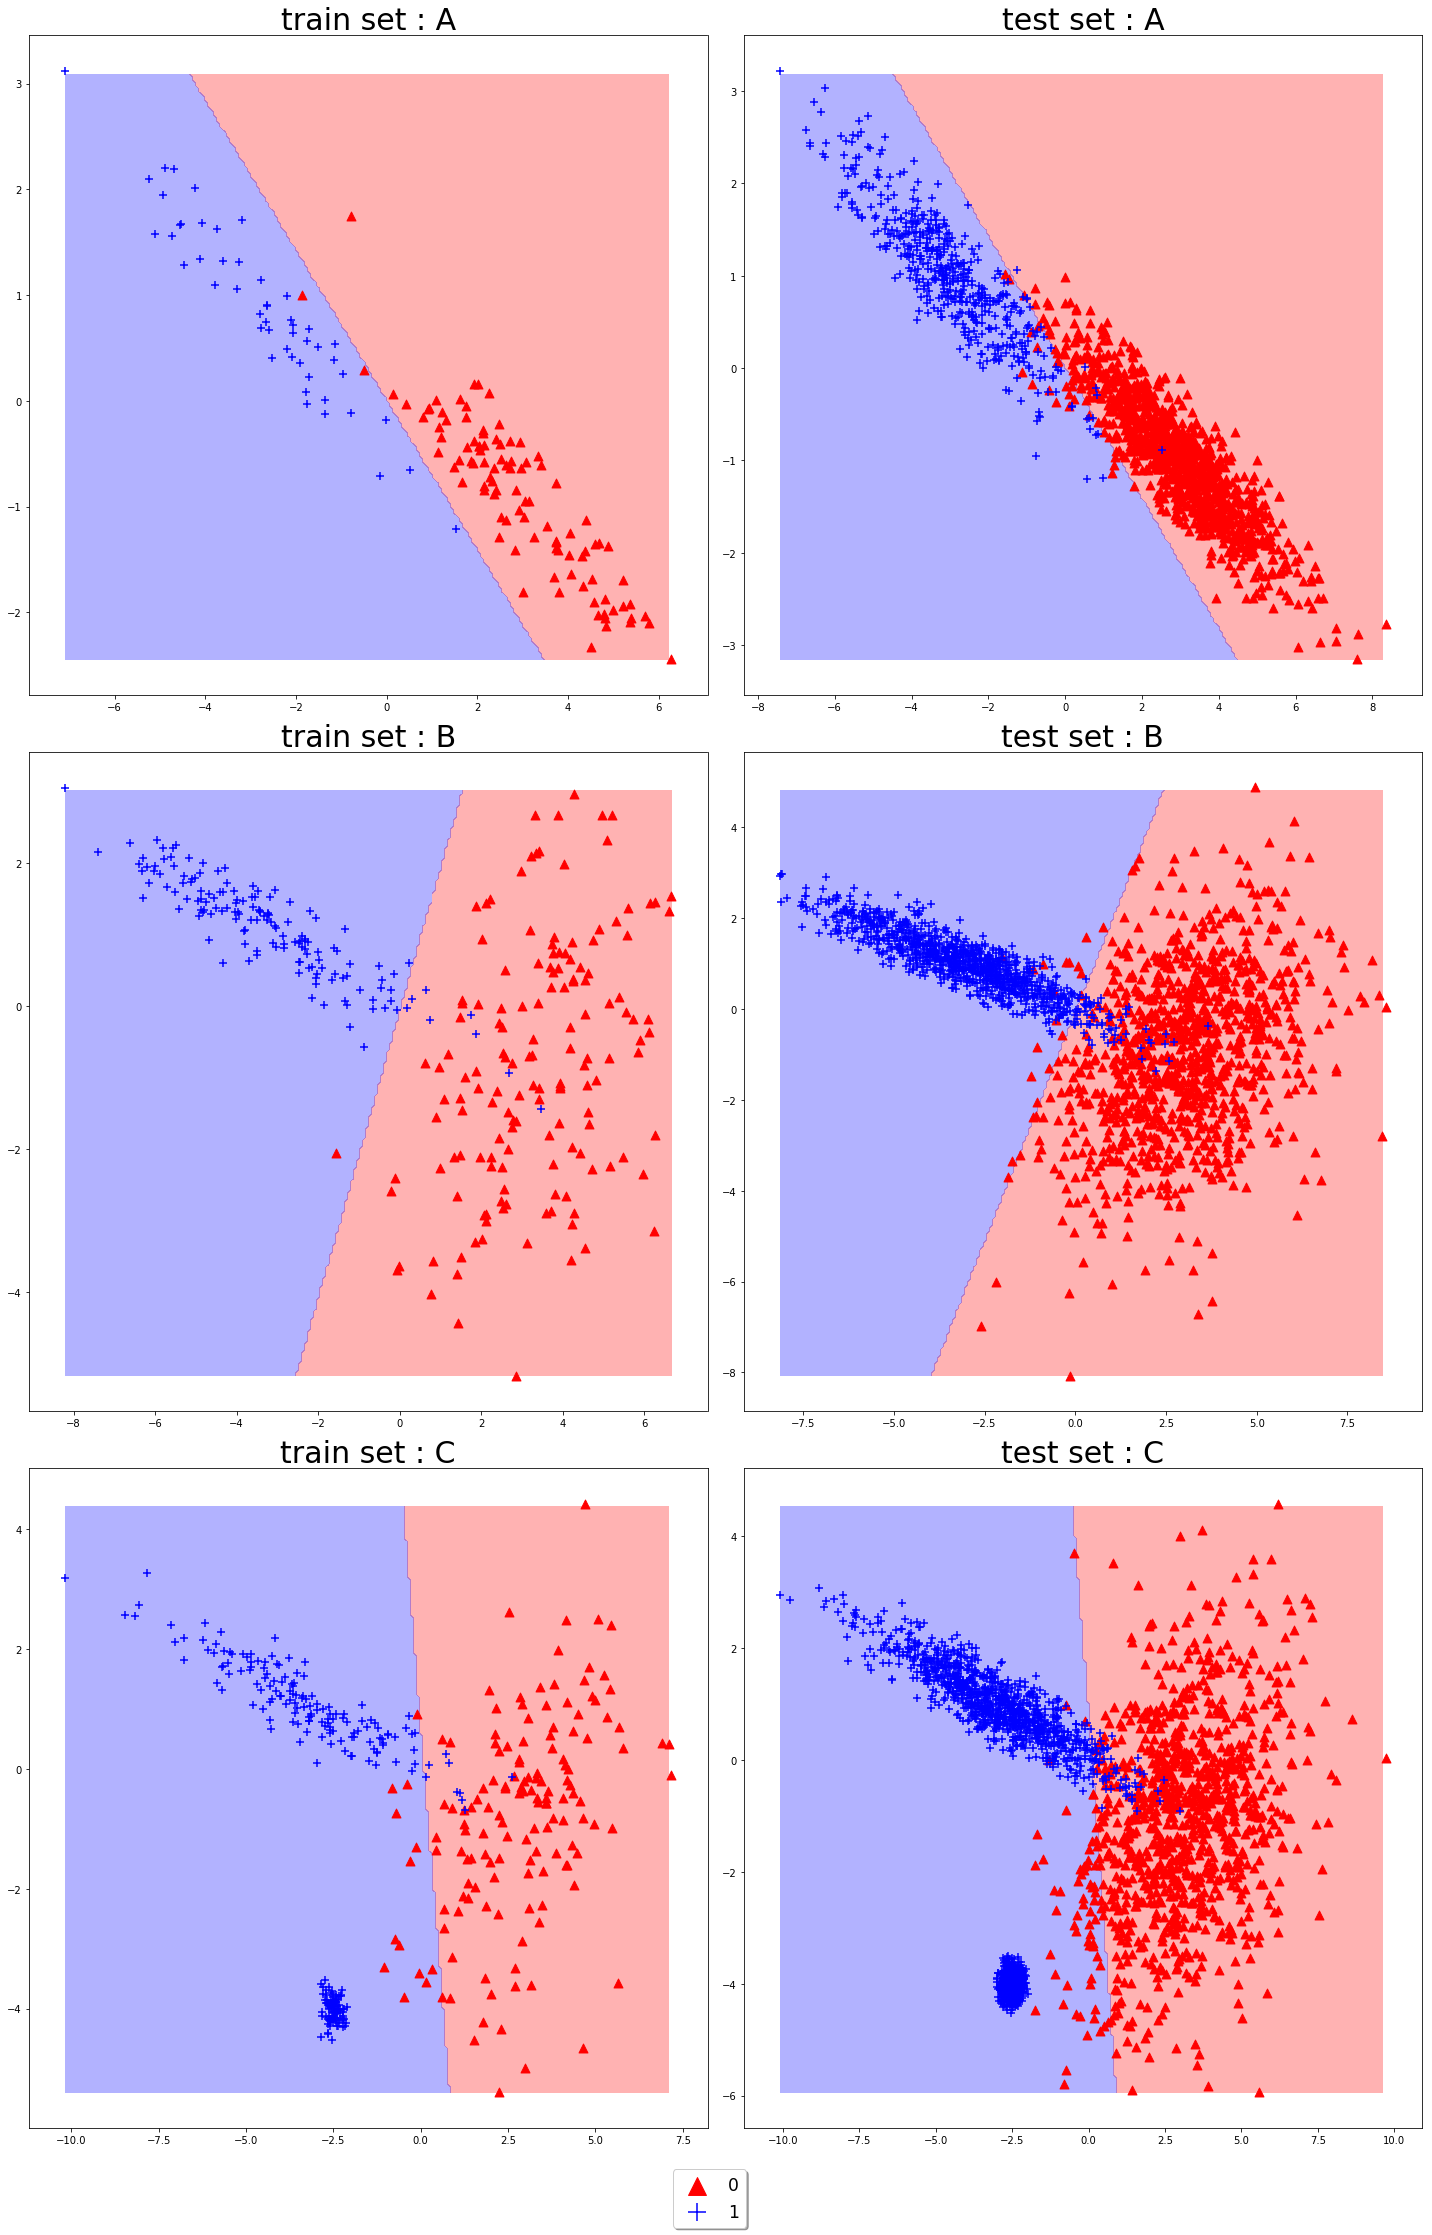
\includegraphics[height = 0.9\textheight]{LDA}
	\caption{Représentation graphique obtenue pour le modèle LDA sur les 3 jeux de données A, B, C respectivement de en haut en bas. Sur la colonne de gauche, les sous-ensembles d'entrainement. Sur la colonne de droite les sous-ensembles de test. La courbe de transition de la classe bleue à la classe rouge est définie par l'équation \( p(y = 1 | x) = 0.5\)}
	\label{fig:LDA}
\end{figure}

\subsection{Logistic regression}

\begin{table}[H]
	\centering
	\begin{tabular}{|L{3cm} || C{2cm} | C{3cm} |}
		\hline
		\rowcolor{maroon!10}
		Jeu de données d'entraînement & \( \widehat{\omega_{MLE}} \)   & \( \widehat{b_{MLE}} \) \\\hline
		A                             & \(\begin{pmatrix}-16.2\\ -27.2 \end{pmatrix}\) & -3.09                   \\\hline
		B                             & \(\begin{pmatrix}-1.71\\ 1.02 \end{pmatrix}\) & 1.35                    \\\hline
		C                             & \(\begin{pmatrix}-2.20\\ 0.709 \end{pmatrix}\) & 0.959                   \\\hline
	\end{tabular}
	\caption{Valeurs numériques des estimateurs MLE obtenus par IRLS du modèle de régression logistique}
	\label{tab:logistic}
\end{table}

Les résultats numériques obtenus pour les estimateurs pour le modèle de régression lgositique sont présentés en Table~\ref{tab:logistic}, Graphiquement, on représente également en Figure~\ref{fig:logistic} les zones de \( \R^2 \) en deux couleurs suivant la classe attribuée par le modèle de régression logsitique déterminé.

\begin{figure}[H]
	\centering
	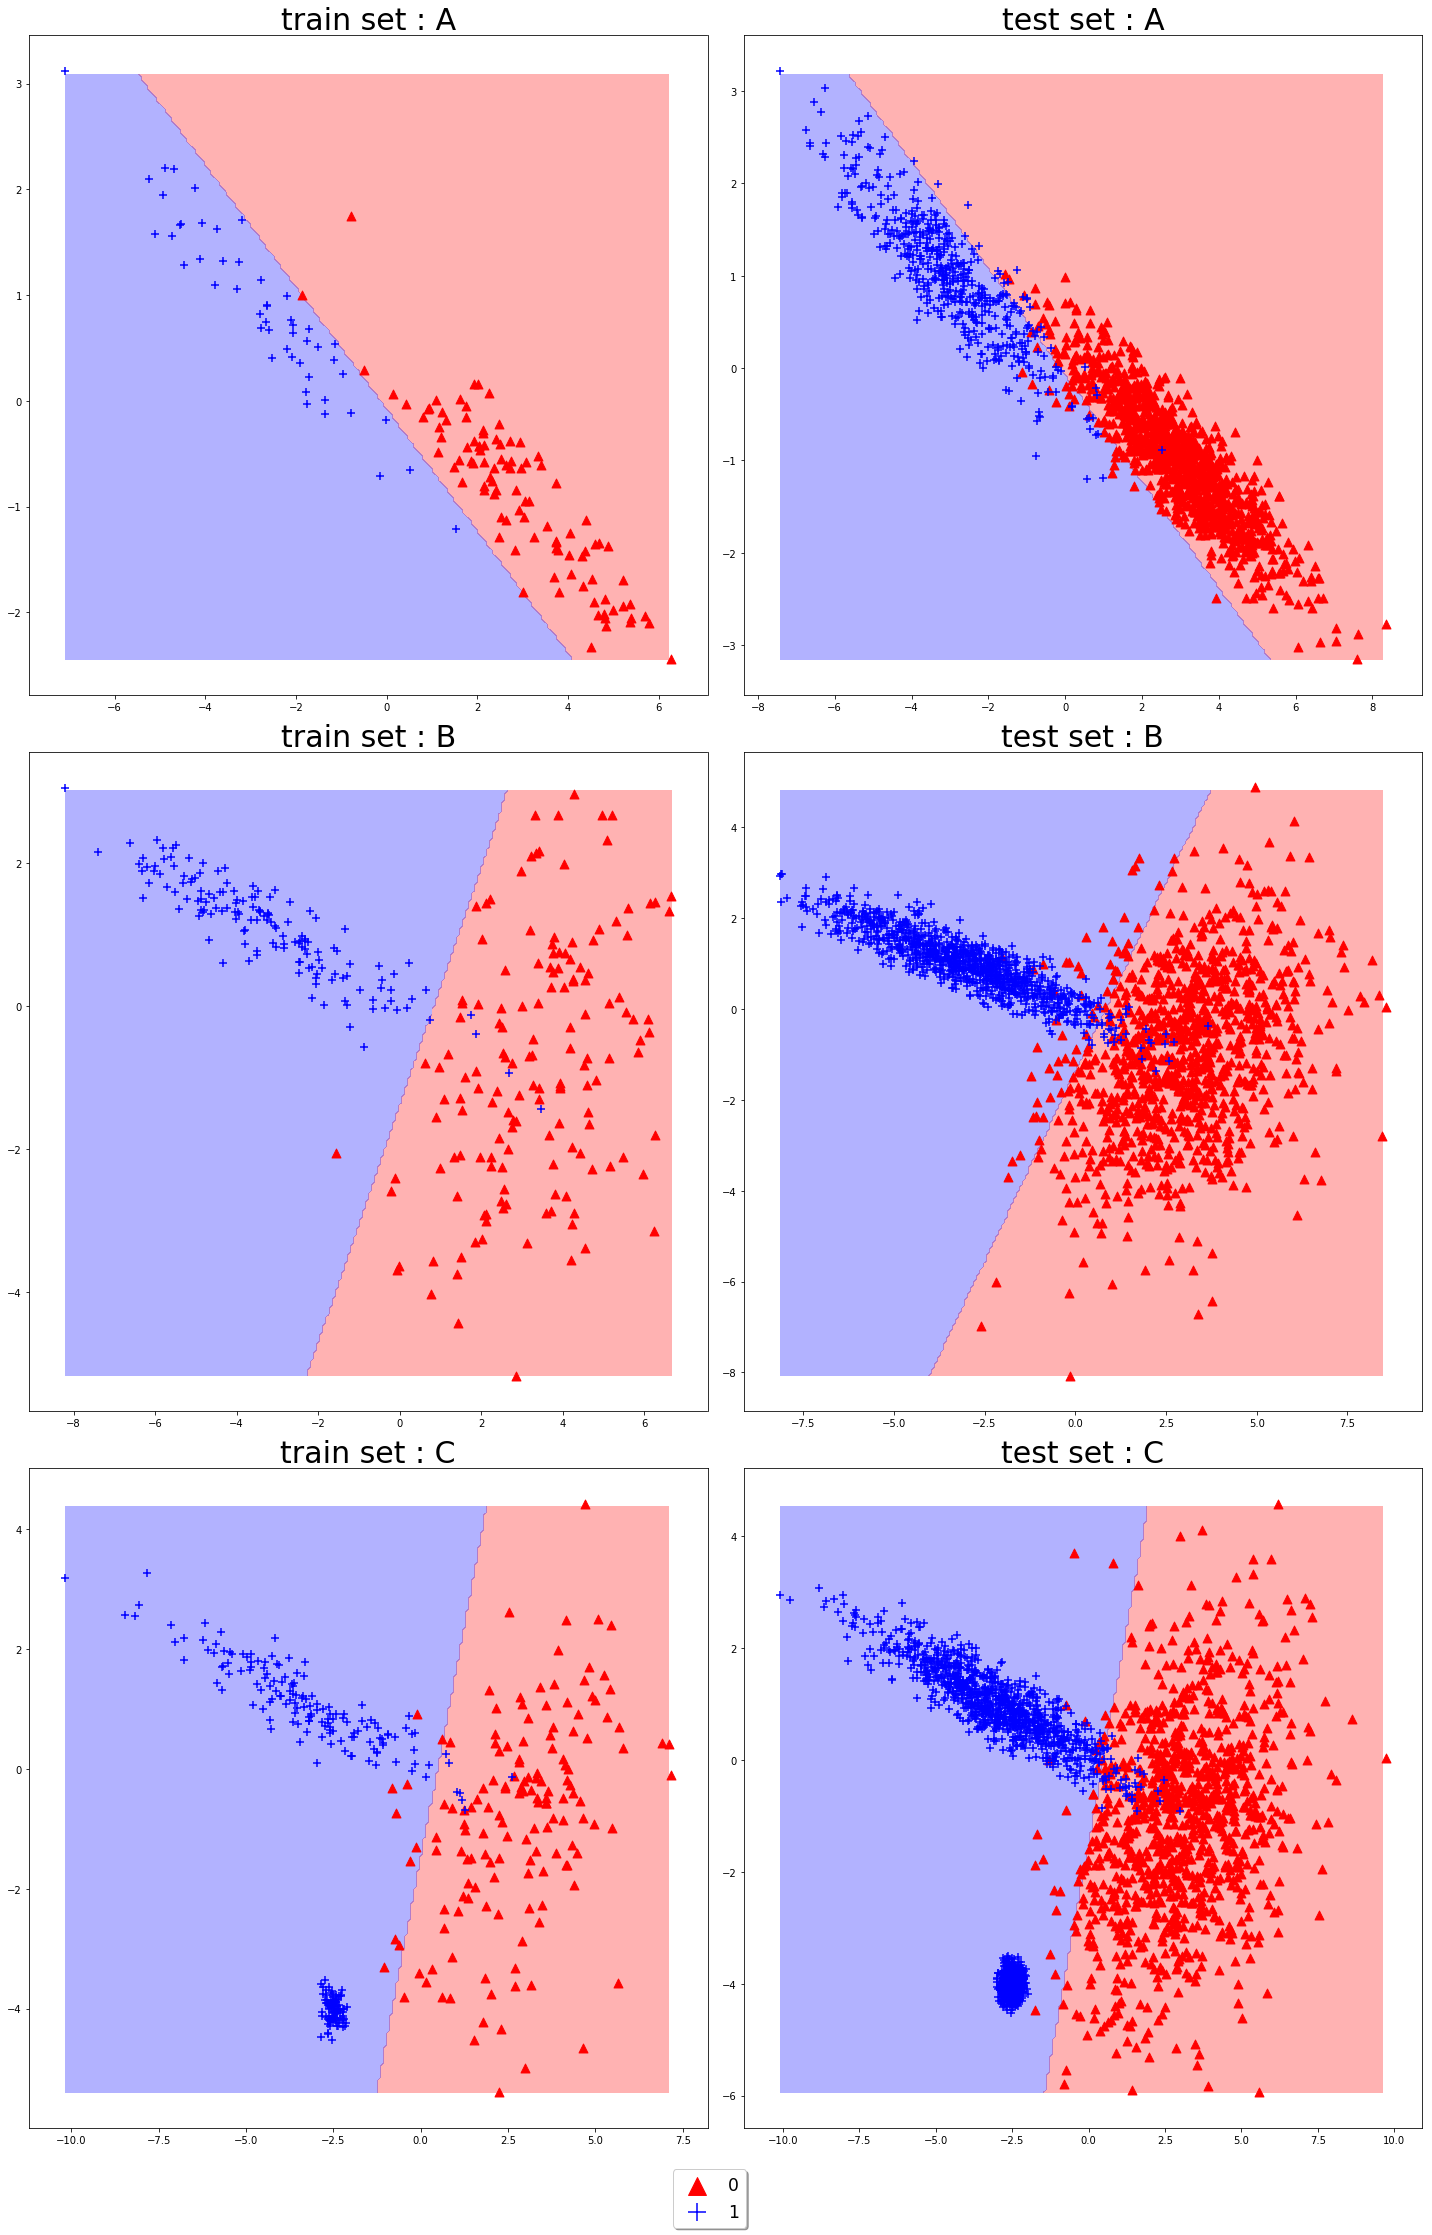
\includegraphics[height = 0.9\textheight]{logistic}
	\caption{Représentation graphique obtenue pour le modèle de régression logistique sur les 3 jeux de données A, B, C respectivement de en haut en bas. Sur la colonne de gauche, les sous-ensembles d'entrainement. Sur la colonne de droite les sous-ensembles de test. La courbe de transition de la classe bleue à la classe rouge est définie par l'équation \( p(y = 1 | x) = 0.5\)}
	\label{fig:logistic}
\end{figure}

\subsection{Linear regression}

\begin{table}[H]
	\centering
	\begin{tabular}{|L{3cm} || C{3cm} | C{3cm} | C{4cm}|}
		\hline
		\rowcolor{maroon!10}
		Jeu de données d'entraînement & \( \widehat{\omega_{MLE}} \)   & \( \widehat{b_{MLE}} \) & \( \widehat{\sigma^2_{MLE}} \) \\\hline
		A                             & \(\begin{pmatrix}-0.264\\ -0.373 \end{pmatrix}\) & \(0.492\)               & \( 0.0399\)                    \\\hline
		B                             & \(\begin{pmatrix}-0.104\\ 0.0518 \end{pmatrix}\) & \(0.500\)               & 0.0543                         \\\hline
		C                             & \(\begin{pmatrix}-0.128\\ -0.0170 \end{pmatrix}\) & \(0.508\)               & \( 0.0622\)                    \\\hline
	\end{tabular}
	\caption{Valeurs numériques des estimateurs MLE obtenus par les équations normales du modèle de régression linéaire}
	\label{tab:linear}
\end{table}

Les résultats numériques obtenus pour les estimateurs pour le modèle de régression linéaire sont présentés en Table~\ref{tab:linear}, Graphiquement, on représente également en Figure~\ref{fig:linear} les zones de \( \R^2 \) en deux couleurs suivant la classe attribuée par le modèle de régression logsitique déterminé. La courbe de séparation pour \( p(y = 1 | x) = 0.5\) n'est plus linéaire comme précédemment du fait de la forme quadratique qui intervient dans cette probabilité qui suit une loi de distribution gaussienne \( \sim N(\omega^{\intercal} X + b, \sigma^2)\)

\begin{figure}[H]
	\centering
	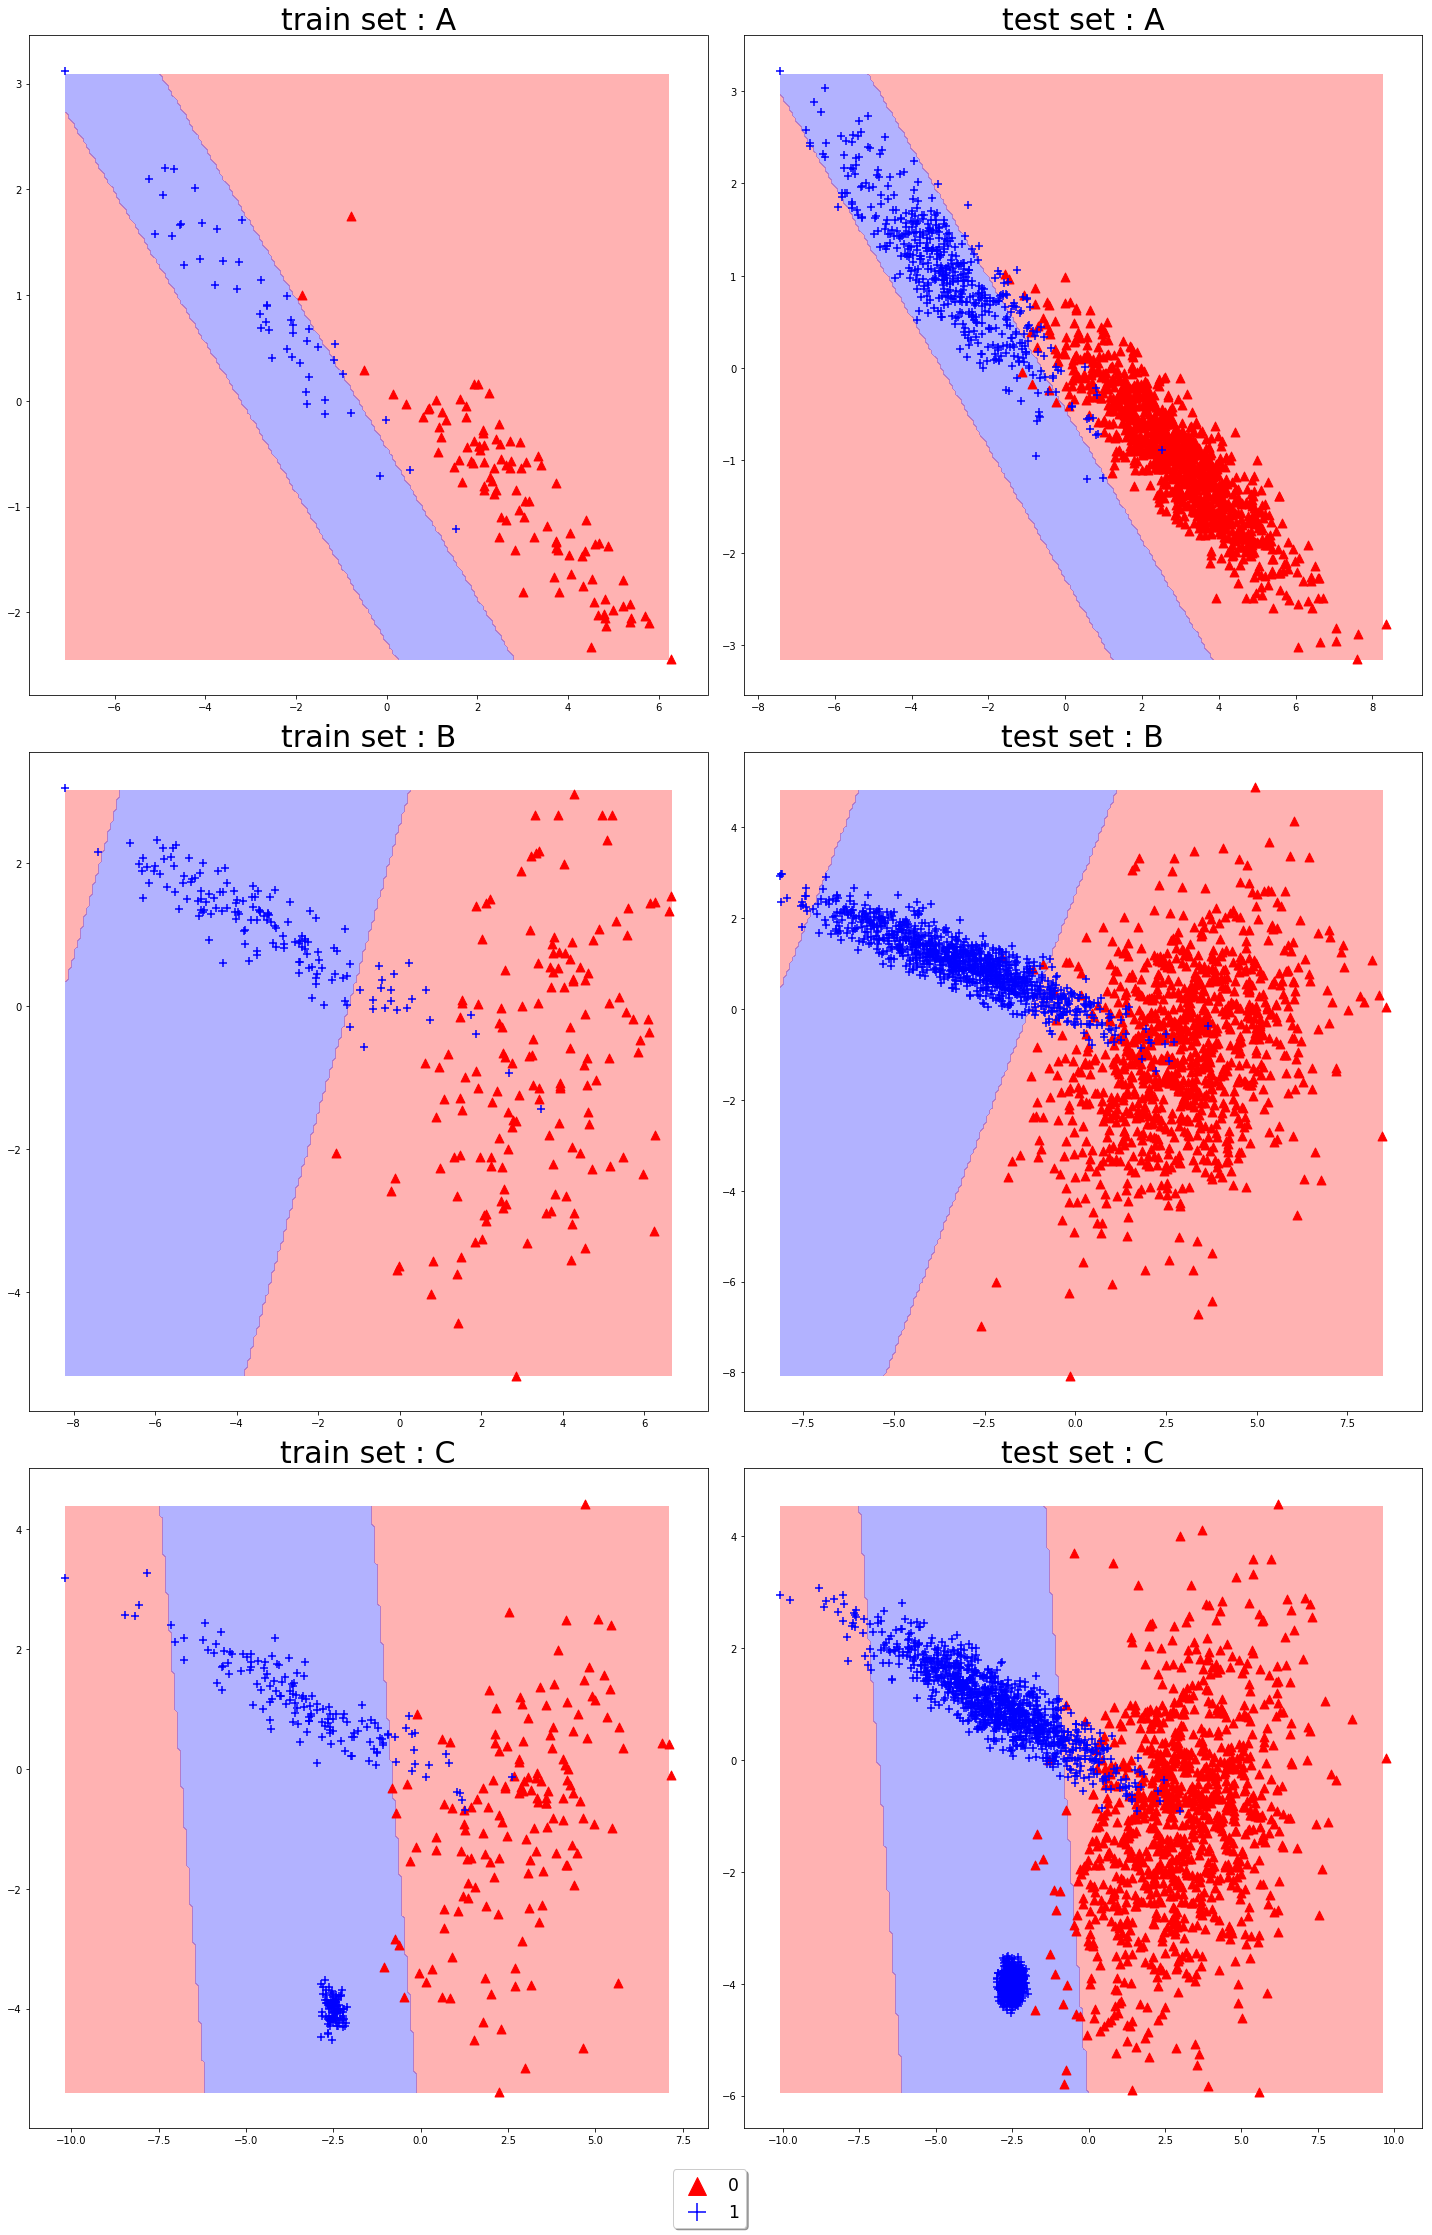
\includegraphics[height = 0.9\textheight]{linear}
	\caption{Représentation graphique obtenue pour le modèle de régression linéaire sur les 3 jeux de données A, B, C respectivement de en haut en bas. Sur la colonne de gauche, les sous-ensembles d'entrainement. Sur la colonne de droite les sous-ensembles de test. La courbe de transition de la classe bleue à la classe rouge est définie par l'équation \( p(y = 1 | x) = 0.5\)}
	\label{fig:linear}
\end{figure}

\subsection{Compare previous models}

\begin{table}[H]
	\centering
	\begin{tabular}{|L{2cm}||C{2cm}|C{2cm}|C{2cm}|C{2cm}|C{2cm}|C{2cm}|}
		\hline \rowcolor{maroon!10}
		Modèle                & A train & A test & B train & B test & C train & C test \\\hline
		LDA                   & 0.0133  & 0.0200 & 0.0300  & 0.0415 & 0.0550  & 0.0423 \\\hline
		Régression logistique & 0.000   & 0.0326 & 0.0200  & 0.0430 & 0.0400  & 0.0227 \\\hline
		Régression linéaire   & 0.0400  & 0.0473 & 0.0800  & 0.0965 & 0.0725  & 0.0610 \\\hline
	\end{tabular}
	\caption{Erreur de classification de chacun des trois modèles précédemment présentés, sur chaque jeu de données d'apprentissage (train) et de test.}
	\label{tab:2.4}
\end{table}

L'erreur de classification en entraînement et en test a été calculée et est présentée en Table~\ref{tab:2.4}. D'après cette table, on constate que :
\begin{enumerate}
	\item A une exception près (qui est la régression logistique sur C test), l'erreur en apprentissage est moindre qu'en test. Cela va de soi, puisque les estimateurs sont construits de sorte à maximiser la vraisemblance des observations déjà effectuées, et non pas celles qui ne l'ont pas encore été.
	\item La LDA et la régression linéaire donne des erreurs similaires en test et en apprentissage, tandis que la régression logistique a tantôt une erreur nulle en apprentissage mais pas en test, tantôt une erreur similaire en apprentissage et en test, tantôt une erreur plus faible en test qu'en apprentissage. Cela s'explique par le fait que la régression logistique n'est parfaitement capable que de séparer des données linéairement séparables.
	\item Sur le premier jeu de données, linéairement séparables en apprentissage, la régression logistique donne une erreur nulle. La LDA donne une erreur entre \( 1~\%\) en apprentissage et \(2~\%\) en test, stable avec la multiplication de données à la frontière de décision. La stabilité et la relative performance s'expliquent par la vérification de l'hypothèse de distribution des données suivant deux gaussiennes très étirées, avec peu de recoupement. La régression linéaire, pour sa part, donne des résultats toujours substenciellement moins bons. Le jeu de données C ne peut plus raisonnablement être considéré comme issus de la distribution de deux gaussiennes
\end{enumerate}

\subsection{QDA model}

\begin{table}[H]
	\centering
	\begin{tabular}{|L{1.5cm} || C{1cm} | C{2cm} | C{2cm} | C{3.3cm}| C{3.3cm} |}
		\hline
		\rowcolor{maroon!10}
		Jeu de données d'entraînement & \( \widehat{\uppi_{MLE}} \) & \( \widehat{\mu_{0, MLE}} \)   & \( \widehat{\mu_{1, MLE}} \)   & \(\widehat{\Sigma_{0, MLE}}\)  & \(\widehat{\Sigma_{1, MLE}}\)  \\\hline
		A                             & \( 0.333 \)                 & \(\begin{pmatrix}2.89\\ -0.984 \end{pmatrix}\) & \(\begin{pmatrix}-2.69\\ 0.866\end{pmatrix}\) & \(\begin{pmatrix}2.31 & -1.05 \\-1.05 & 0.576\\\end{pmatrix}\) & \(\begin{pmatrix}2.70 & -1.30 \\-1.30 & 0.690\\\end{pmatrix}\) \\\hline
		B                             & \( 0.500 \)                 & \(\begin{pmatrix}3.34\\ -0.835 \end{pmatrix}\) & \(\begin{pmatrix}-3.22\\ 1.08\end{pmatrix}\) & \(\begin{pmatrix}3.35 & -0.135 \\-0.135 & 1.74\\\end{pmatrix}\) & \(\begin{pmatrix}4.15 & -1.33 \\-1.33 & 0.516\\\end{pmatrix}\) \\\hline
		C                             & \( 0.625 \)                 & \(\begin{pmatrix}2.79\\ -0.838 \end{pmatrix}\) & \(\begin{pmatrix}-2.94\\ -0.958\end{pmatrix}\) & \(\begin{pmatrix}2.90 & 1.24 \\ 1.24 & 2.92\\\end{pmatrix}\) & \(\begin{pmatrix}2.87 & -1.76 \\-1.76 & 6.56\\\end{pmatrix}\) \\\hline
	\end{tabular}
	\caption{Valeurs numériques des estimateurs MLE du modèle LDA}
	\label{tab:QDA}
\end{table}

Les résultats numériques obtenus pour les estimateurs pour le modèle de régression linéaire sont présentés en Table~\ref{tab:QDA}, Graphiquement, on représente également en Figure~\ref{fig:QDA} les zones de \( \R^2 \) en deux couleurs suivant la classe attribuée par le modèle de régression logsitique déterminé. La courbe de séparation pour \( p(y = 1 | x) = 0.5\) n'est plus linéaire comme précédemment dans le modèle LDA du fait de la forme quadratique qui intervient dans cette probabilité.

\begin{figure}[H]
	\centering
	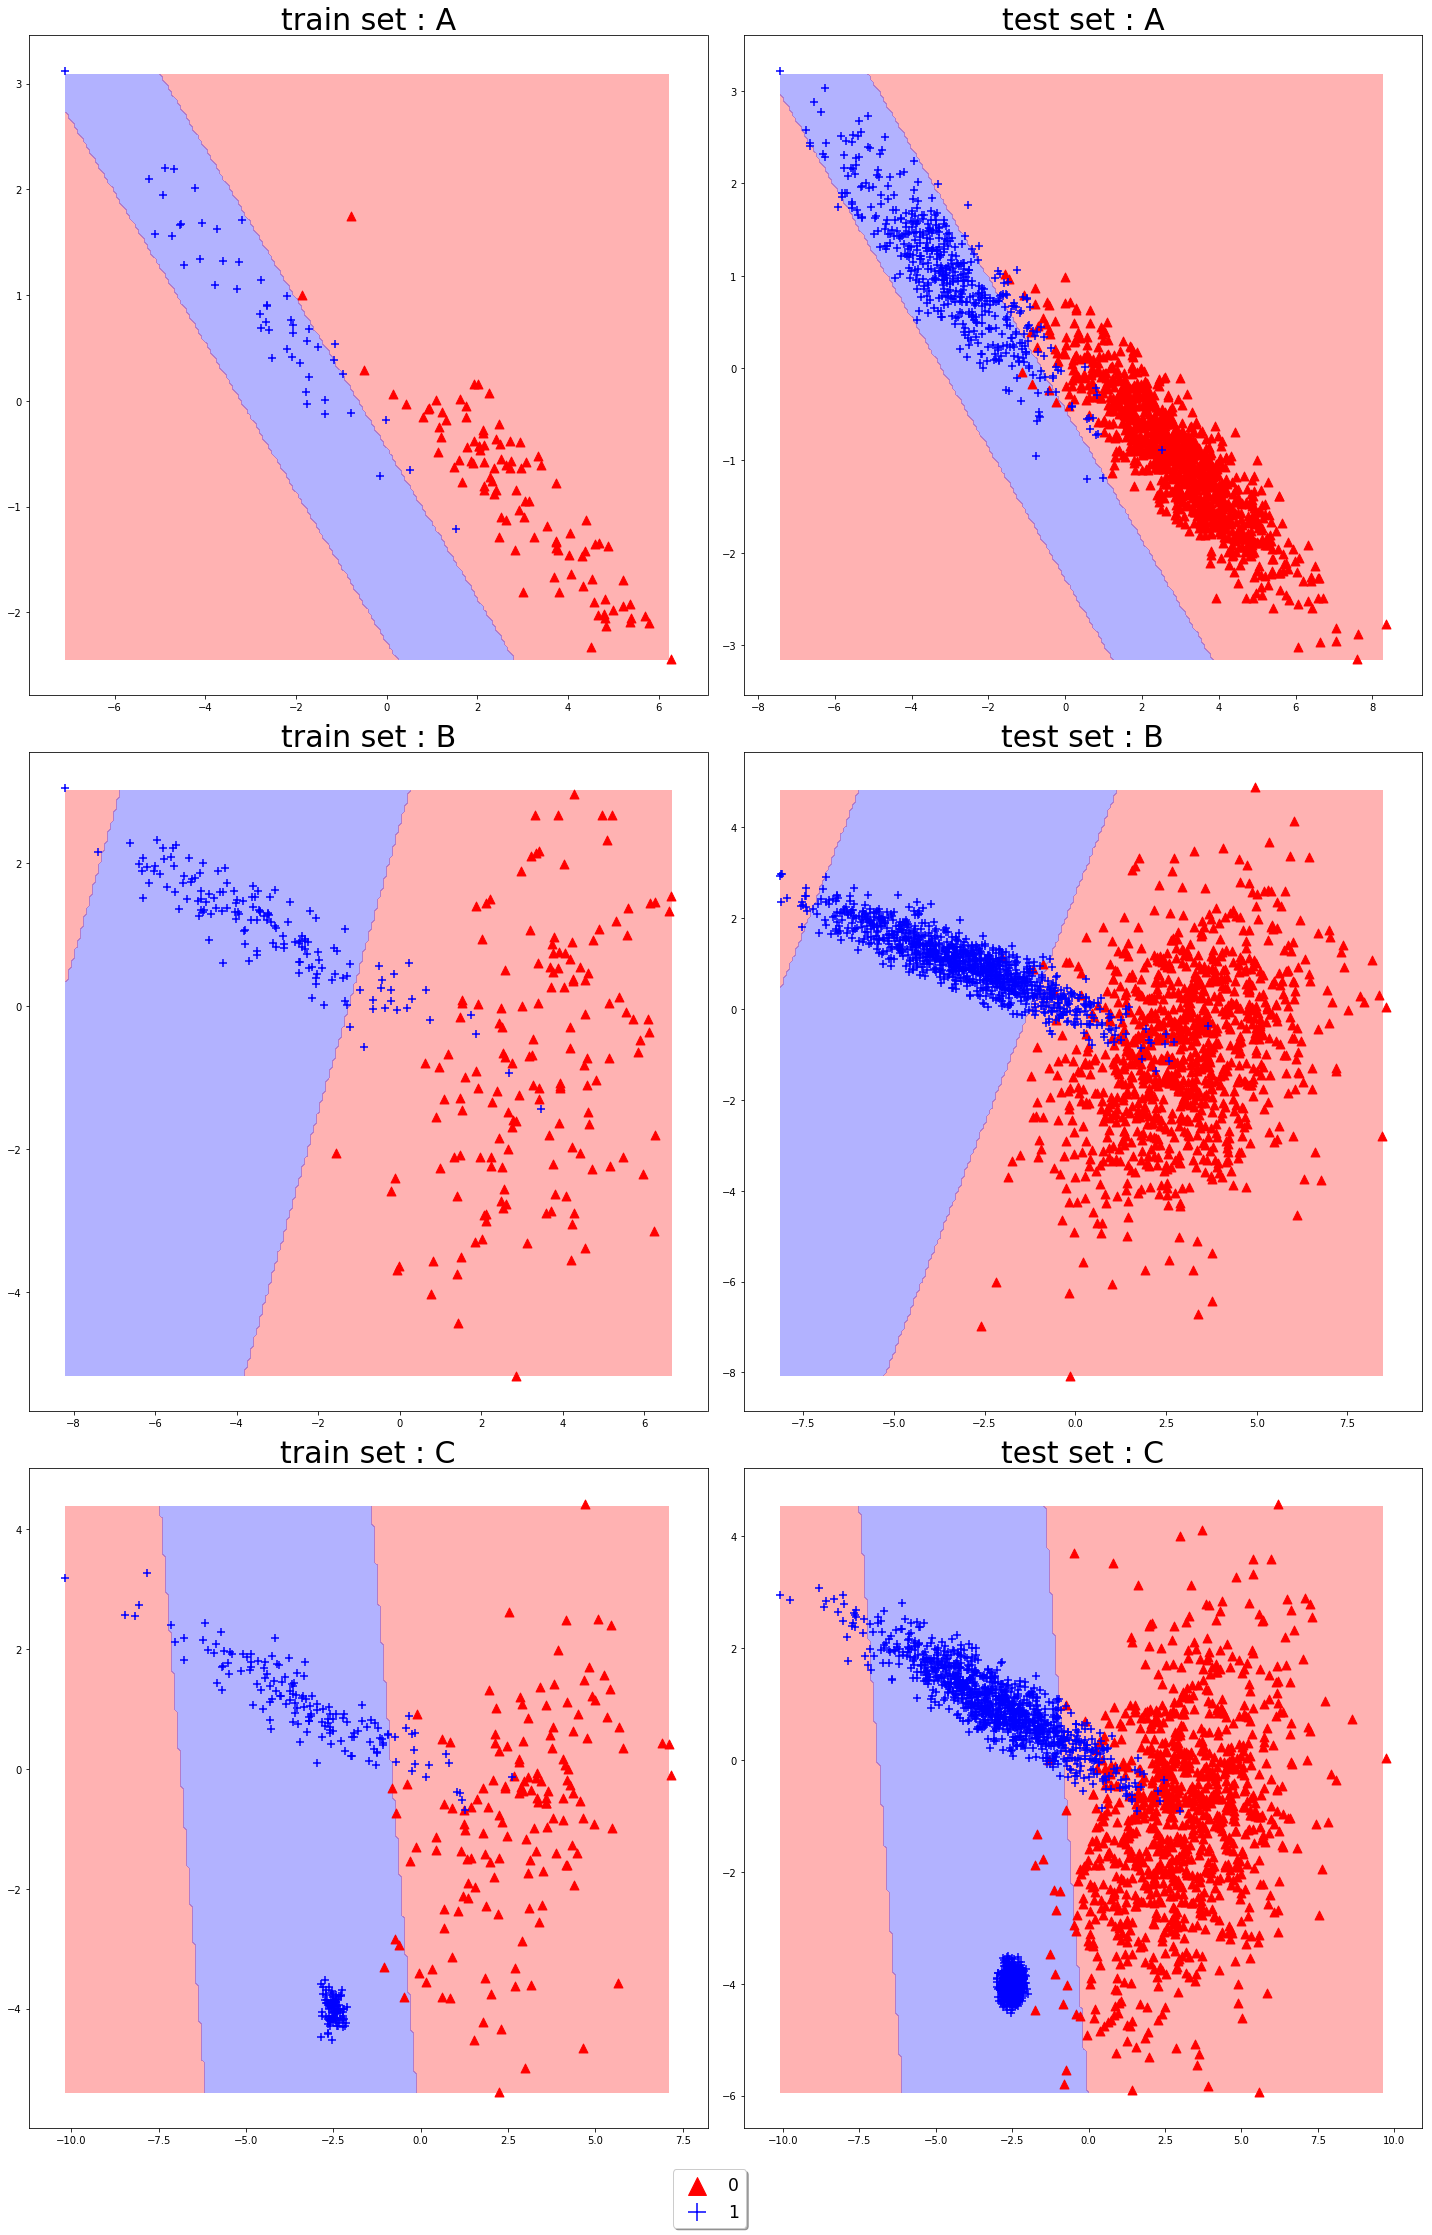
\includegraphics[height = 0.9\textheight]{linear}
	\caption{Représentation graphique obtenue pour le modèle QDA sur les 3 jeux de données A, B, C respectivement de en haut en bas. Sur la colonne de gauche, les sous-ensembles d'entrainement. Sur la colonne de droite les sous-ensembles de test. La courbe de transition de la classe bleue à la classe rouge est définie par l'équation \( p(y = 1 | x) = 0.5\)}
	\label{fig:QDA}
\end{figure}
\end{document}
